% ══════════════════════════════════════════════════════════════════
% Apple-inspired academic poster — space, light, precision
% LAYOUT: 3-Act Integrated Flow (Claim -> Inline Visual Proof)
% ══════════════════════════════════════════════════════════════════
\documentclass[25pt, a0paper, landscape]{tikzposter}

% ── Typography: Helvetica system, Palatino math ──
\usepackage[utf8]{inputenc}
\usepackage[T1]{fontenc}
\usepackage{mathpazo}
\usepackage[scaled=0.94]{helvet}
\renewcommand{\familydefault}{\sfdefault}
\renewcommand{\rmdefault}{ppl}

% ── Packages ──
\usepackage{amsmath,amssymb,amsthm}
\usepackage{bm}
\usepackage{graphicx}
\usepackage{booktabs}
\usepackage{enumitem}
\usepackage{url}
\usepackage{xcolor}
\usepackage{qrcode}
\usepackage{microtype}
\usepackage{fontawesome}
\usepackage{tikz}
\usetikzlibrary{arrows.meta, positioning, calc, fit, backgrounds}

% ── Paths / macros ──
\graphicspath{{./images/}{./figures/}{./elements/}{./}}
\newcommand{\Loss}{\mathcal{L}}
\newcommand{\er}{\mathrm{er}_2}
\newcommand{\T}{T_\theta}

% ══════════════════════════════════════════════════════════════════
% COLOR SYSTEM
% ══════════════════════════════════════════════════════════════════
\definecolor{spaceblack}{RGB}{29, 29, 31}
\definecolor{primary}{RGB}{29, 29, 31}
\definecolor{secondary}{RGB}{62, 62, 66}
\definecolor{tertiary}{RGB}{130, 130, 136}
\definecolor{accent}{RGB}{45, 62, 95}         
\definecolor{accentsoft}{RGB}{240, 240, 238}  
\definecolor{canvas}{RGB}{248, 248, 248}
\definecolor{card}{RGB}{255, 255, 255}
\definecolor{separator}{RGB}{210, 210, 212}
\definecolor{frozen}{RGB}{168, 50, 42}        
\definecolor{cloned}{RGB}{35, 82, 160}        
\definecolor{escape}{RGB}{38, 115, 52}        
\definecolor{myyellow}{RGB}{170, 132, 35}
\definecolor{takeawaybg}{RGB}{240, 247, 240}  
\definecolor{myplane}{RGB}{240, 240, 242}
\definecolor{mygrid}{RGB}{225, 225, 228}
\definecolor{mygray}{RGB}{142, 142, 147}

% ══════════════════════════════════════════════════════════════════
% THEME & STYLES
% ══════════════════════════════════════════════════════════════════
\tikzposterlatexaffectionproofoff
\usetheme{Default}
\usecolorstyle{Default}
\colorlet{backgroundcolor}{canvas}

\defineblockstyle{Apple}{
    titlewidthscale=1, bodywidthscale=1,
    titleleft, titleoffsetx=0pt, titleoffsety=0pt,
    bodyoffsetx=0pt, bodyoffsety=0pt,
    bodyverticalshift=0pt, roundedcorners=8,
    linewidth=0pt,
    titleinnersep=10pt, bodyinnersep=14pt
}{
    \fill[card, rounded corners=\blockroundedcorners]
      (blockbody.south west) rectangle (blocktitle.north east);
    \fill[accent!80!black, rounded corners=2pt]
      ([yshift=-1pt]blocktitle.north west) rectangle
      ([yshift=-3.5pt]blocktitle.north east);
    \draw[separator, line width=0.5pt]
      ([yshift=2pt]blockbody.north west) -- ([yshift=2pt]blockbody.north east);
}
\useblockstyle{Apple}

\colorlet{blocktitlebgcolor}{card}
\colorlet{blocktitlefgcolor}{primary}
\colorlet{blockbodybgcolor}{card}
\colorlet{blockbodyfgcolor}{secondary}

\definetitlestyle{SpaceBlack}{
    width=\paperwidth, roundedcorners=0, linewidth=0pt,
    innersep=22pt, titletotopverticalspace=0mm,
    titletoblockverticalspace=12mm
}{
    \begin{scope}[line width=0pt]
    \draw[draw=none, fill=spaceblack]
      (\titleposleft,\titleposbottom) rectangle (\titleposright,\titlepostop);
    \end{scope}
}
\usetitlestyle{SpaceBlack}
\colorlet{titlebgcolor}{spaceblack}
\colorlet{titlefgcolor}{white}

% ── Macros ──
\newcommand{\resultbox}[1]{%
\begin{tikzpicture}
\node[fill=accentsoft, inner sep=12pt, text width=0.92\linewidth,
      rounded corners=4pt, font=\large] (box) {#1};
\fill[accent, rounded corners=1pt]
  ([xshift=0pt]box.north west) rectangle ([xshift=2.5pt]box.south west);
\end{tikzpicture}%
}
\newcommand{\takeawaybox}[1]{%
\begin{tikzpicture}
\node[fill=takeawaybg, inner sep=12pt, text width=0.92\linewidth,
      rounded corners=4pt, font=\large] (box) {#1};
\fill[escape!70!black, rounded corners=1pt]
  ([xshift=0pt]box.north west) rectangle ([xshift=2.5pt]box.south west);
\end{tikzpicture}%
}
\newcommand{\seclabel}[1]{{\small\color{tertiary}\MakeUppercase{#1}}\\[3pt]}
\newcommand{\thinrule}{\vspace{2mm}{\color{separator}\hrule height 0.4pt}\vspace{3mm}}

% ══════════════════════════════════════════════════════════════════
\begin{document}

% ── Title ──
\title{\textbf{Barriers for Learning in an Evolving World: Mathematical Understanding of Loss of Plasticity}}

\author{{\Large%
Amir Joudaki$^{1}$,\;
Giulia Lanzillotta$^{1}$,\;
Mohammad Samragh Razlighi$^{2}$,\;
Iman Mirzadeh$^{2}$,\;
Keivan Alizadeh$^{2}$,\;
Thomas Hofmann$^{1}$,\;
Mehrdad Farajtabar$^{2}$,\;
Fartash Faghri$^{2}$%
}\\[4pt]
{\large $^{1}$ETH Z\"urich \quad $^{2}$Apple \quad
\texttt{amir.joudaki@inf.ethz.ch}}%
}

\institute{}

\maketitle

% ══════════════════════════════════════════════════════════════════
% BODY — 3 THEMATIC COLUMNS (Concept -> Trap -> Cause/Cure)
% ══════════════════════════════════════════════════════════════════
\begin{columns}

% ──────────────────────────────────────────────────────────────────
% COLUMN 1 — The Phenomenon
% ──────────────────────────────────────────────────────────────────
\column{0.32}

\block{\textbf{1. The Phenomenon}}{
\large
\seclabel{Continual Learning \& Loss of Plasticity}
Deep learning excels on fixed datasets. In continual learning {\small[1,\,2]}, models suffer from \textbf{Loss of Plasticity (LoP)} {\small[3,\,4]}: past knowledge is retained, but the ability to fit \emph{future} data degrades severely.

\vspace{2mm}
\seclabel{Symptoms}
Across architectures, \textcolor{frozen}{dead units} {\small[5]} and \textcolor{cloned}{duplicate features} {\small[6]} accumulate while effective rank collapses.

\vspace{3mm}
\begin{center}
\begin{minipage}[c]{0.45\linewidth}\centering
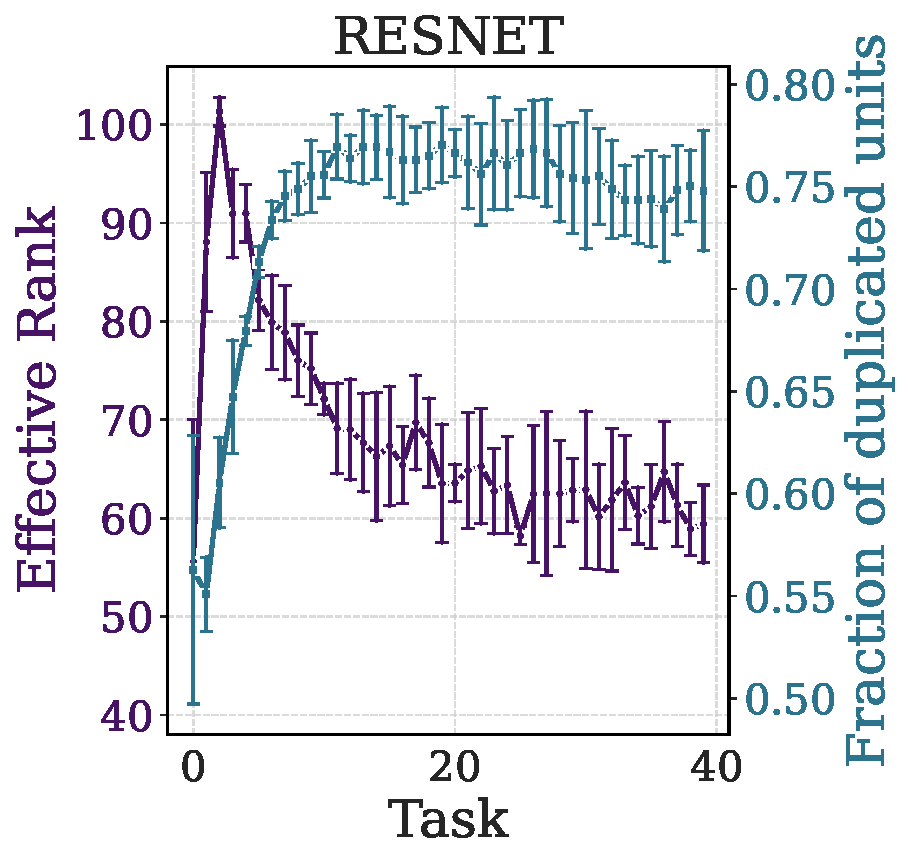
\includegraphics[width=\linewidth]{images/resnet_block_rankdead_plot.pdf}
\end{minipage}
\hspace{6mm}
\begin{minipage}[c]{0.38\linewidth}\centering
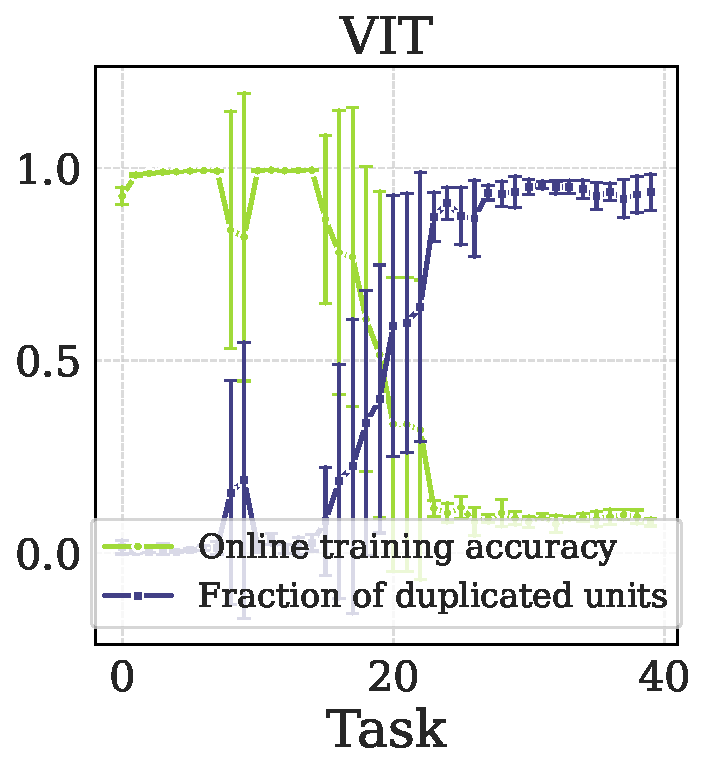
\includegraphics[width=\linewidth]{images/vit_block_dup_fraction_plot.pdf}
\end{minipage}
\end{center}

\vspace{3mm}
Prior work catalogs symptoms but not the \textbf{mechanism of persistence}:

\begin{center}
{\color{accent}\emph{Why does gradient descent fail to recover once the non-plastic state appears?}}
\end{center}
}

\block{\textbf{The Structural Trap: LoP Manifolds}}{
\large
A manifold $\mathcal{M}\subset\Theta$ induces LoP if the gradient is permanently tangent to it:
\[
\nabla_\theta \Loss(\theta)\in \T \mathcal{M} \qquad \forall\, \theta\in\mathcal{M}.
\]

\seclabel{Distribution-independent form}
A stronger, samplewise condition: $\nabla_\theta \ell(\theta;x,y)\in \T \mathcal{M}$, implies invariance under \emph{any} data distribution.

\vspace{2mm}
\resultbox{%
The trap is enforced by the \textbf{network equations}, not by a particular dataset. For affine LoP manifolds, discrete GD/SGD also remains trapped in~$\mathcal{M}$.
}

\vspace{2mm}
\begin{center}
\resizebox{0.85\linewidth}{!}{%
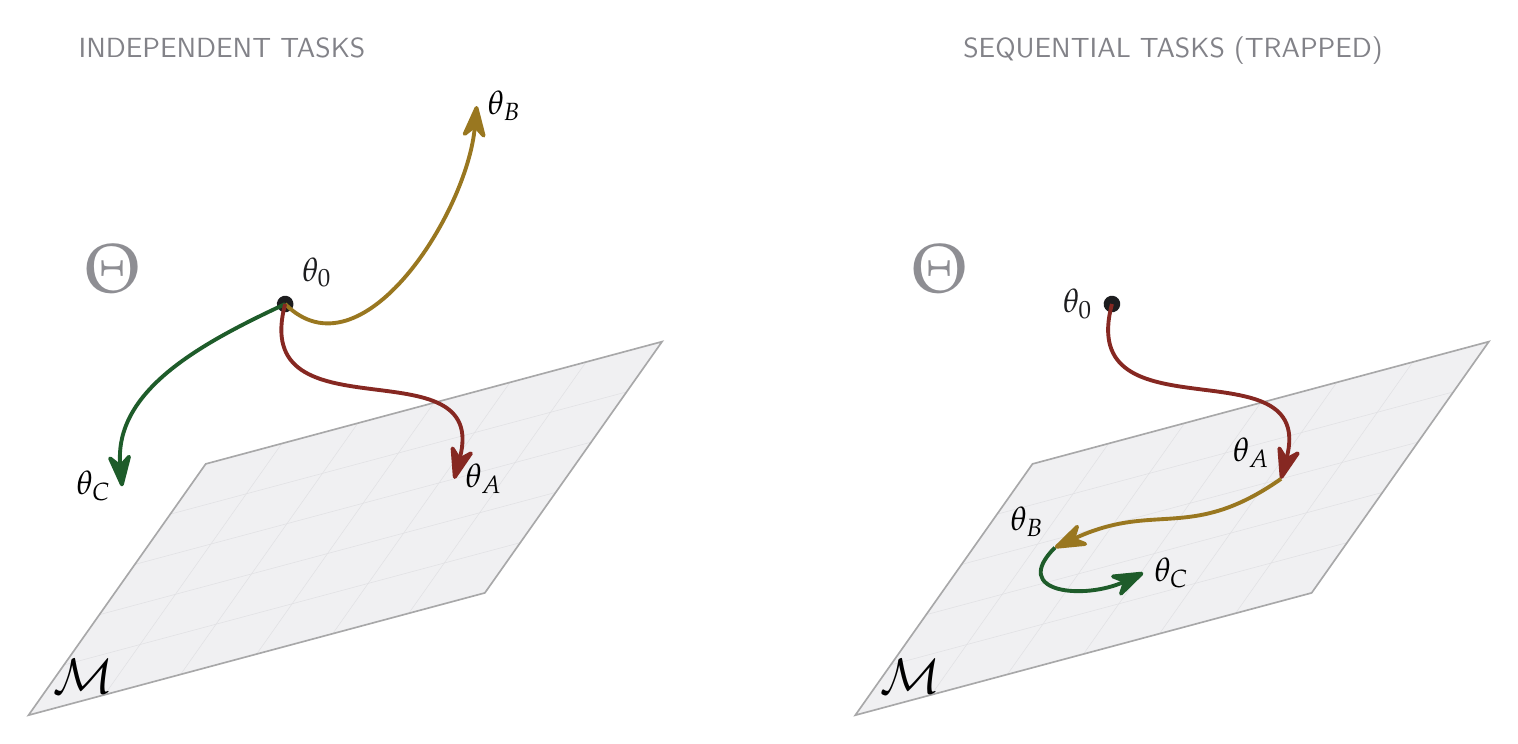
\begin{tikzpicture}[
    >={Stealth[round, length=5mm, width=3.5mm]},
    line width=1.4pt,
    font=\Large,
]
    % --- TOP: Independent Tasks ---
    \begin{scope}[local bounding box=leftpanel,rotate around={15:(4.5, 1.25)}]
        \node[anchor=south, font=\normalsize\color{tertiary}] at (4.5, 7.3) {\MakeUppercase{Independent tasks}};
        \node at (2.5, 5.2) {\Huge \textcolor{mygray}{$\Theta$}};
        \fill[myplane] (0,0) -- (6,0) -- (9,2.5) -- (3,2.5) -- cycle;
        \foreach \i in {1,...,4} { \draw[mygrid, line width=0.2pt] ($(0,0)!\i/5!(3,2.5)$) -- ($(6,0)!\i/5!(9,2.5)$); }
        \foreach \i in {1,...,5} { \draw[mygrid, line width=0.2pt] ($(0,0)!\i/6!(6,0)$) -- ($(3,2.5)!\i/6!(9,2.5)$); }
        \draw[myplane!70!black, line width=0.6pt] (0,0) -- (6,0) -- (9,2.5) -- (3,2.5) -- cycle;
        \node[font=\LARGE\rmfamily] at (0.8, 0.3) {$\mathcal{M}$};
        \coordinate (T0) at (4.5, 4.2);
        \fill[spaceblack] (T0) circle (3pt) node[above right=3pt, font=\large] {$\theta_0$};
        \draw[->, escape!80!black] (T0) to[out=190, in=80, looseness=1.0] (1.9, 2.5) node[left, black, font=\large] {$\theta_C$};
        \draw[->, myyellow!90!black] (T0) to[out=-60, in=-110] (7.5, 6.0) node[right, black, font=\large] {$\theta_B$};
        \draw[->, frozen!80!black] (T0) to[out=-120, in=60,looseness=1.5] (6., 1.5) node[right, black, font=\large] {$\theta_A$};
    \end{scope}
    
    % --- RIGHT: Sequential Tasks ---
    \begin{scope}[xshift=10.5cm, local bounding box=rightpanel,rotate around={15:(4.5, 1.25)}]
        \node[anchor=south, font=\normalsize\color{tertiary}] at (6, 6.8) {\MakeUppercase{Sequential tasks (Trapped)}};
        \node at (2.5, 5.2) {\Huge \textcolor{mygray}{$\Theta$}};
        \fill[myplane] (0,0) -- (6,0) -- (9,2.5) -- (3,2.5) -- cycle;
        \foreach \i in {1,...,4} { \draw[mygrid, line width=0.2pt] ($(0,0)!\i/5!(3,2.5)$) -- ($(6,0)!\i/5!(9,2.5)$); }
        \foreach \i in {1,...,5} { \draw[mygrid, line width=0.2pt] ($(0,0)!\i/6!(6,0)$) -- ($(3,2.5)!\i/6!(9,2.5)$); }
        \draw[myplane!70!black, line width=0.6pt] (0,0) -- (6,0) -- (9,2.5) -- (3,2.5) -- cycle;
        \node[font=\LARGE\rmfamily] at (0.8, 0.3) {$\mathcal{M}$};
        \coordinate (T0s) at (4.5, 4.2);
        \fill[spaceblack] (T0s) circle (3pt) node[left=3pt, font=\large] {$\theta_0$};
        \coordinate (TAs) at (6., 1.5);
        \coordinate (TBs) at (3.0, 1.4);
        \coordinate (TCs) at (4.0, 0.8);
        \draw[->, frozen!80!black] (T0s) to[out=-120, in=60,looseness=1.5] (TAs);
        \node[above left, font=\large] at (TAs) {$\theta_A$};
        \draw[->, myyellow!90!black] (TAs) to[out=-160, in=10, looseness=1.2] (TBs);
        \node[above left, font=\large] at (TBs) {$\theta_B$};
        \draw[->, escape!80!black] (TBs) to[out=210, in=190, looseness=1.8] (TCs);
        \node[right, font=\large] at (TCs) {$\theta_C$};
    \end{scope}
\end{tikzpicture}%
}
\end{center}
}

% ──────────────────────────────────────────────────────────────────
% COLUMN 2 — The Mechanics (Theorem 1)
% ──────────────────────────────────────────────────────────────────
\column{0.34}


\block{\textbf{2. The Mechanics: Exact Traps (Thm 1)}}{
\large

For a LoP manifold $\mathcal{M}\subseteq \Theta$, is \textbf{distribution-independent}, in the sense that for virtually all feasible inputs, regardless of their semantics, the gradient is tangent to the manifold.

\thinrule

\seclabel{Frozen-unit manifold \;$\mathcal{M}_F$}
If units $F\subset V$ are persistently saturated ($f'(z_v(x;\theta))=0$), their incoming gradients vanish for every sample. $\mathcal{M}_F=\bigl\{\theta:\theta_{\mathrm{in}}(v)=\mathrm{const},\ \forall v\in F\bigr\}$.

\vspace{2mm}
{\color{frozen}\rule{14pt}{1.8pt}}\;\; \emph{A frozen unit is permanently silent to backprop.}

\thinrule

\seclabel{Cloning manifold \;$\mathcal{M}_C$}
If block pairs satisfy equal row and column sums:
\[
\textstyle\sum_{v\in S_j}\theta_{uv}=\sum_{v\in S_j}\theta_{u'v},
\quad
\sum_{u\in S_i}\theta_{uv}=\sum_{u\in S_i}\theta_{uv'},
\]
then forward values $h_u(x)=h_{u'}(x)$ and backward errors $\delta_v(x,y)=\delta_{v'}(x,y)$ are strictly identical.

\vspace{2mm}
{\color{cloned}\rule{14pt}{1.8pt}}\;\; \emph{Cloned directions are indistinguishable to both passes.}

\thinrule

\resultbox{%
\textbf{Degeneracy in computation induces degeneracy in the update:}
$(h,\delta) \text{ degenerate} \Rightarrow \text{gradient degenerate} \Rightarrow \nabla_\theta \ell \in \T\mathcal{M}$
}

\thinrule

\seclabel{Empirical Proof: Gradient descent is Trapped}
Do these theoretical locks hold? Yes. If initialized exactly on the cloning manifold, \textbf{counter-intuitively, even Adam is perfectly confined} despite parameter-wise gradient history. 

\vspace{3mm}
\begin{center}
% ROW 1: The Trap (Loss & R2)
\begin{minipage}[c]{0.47\linewidth}\centering
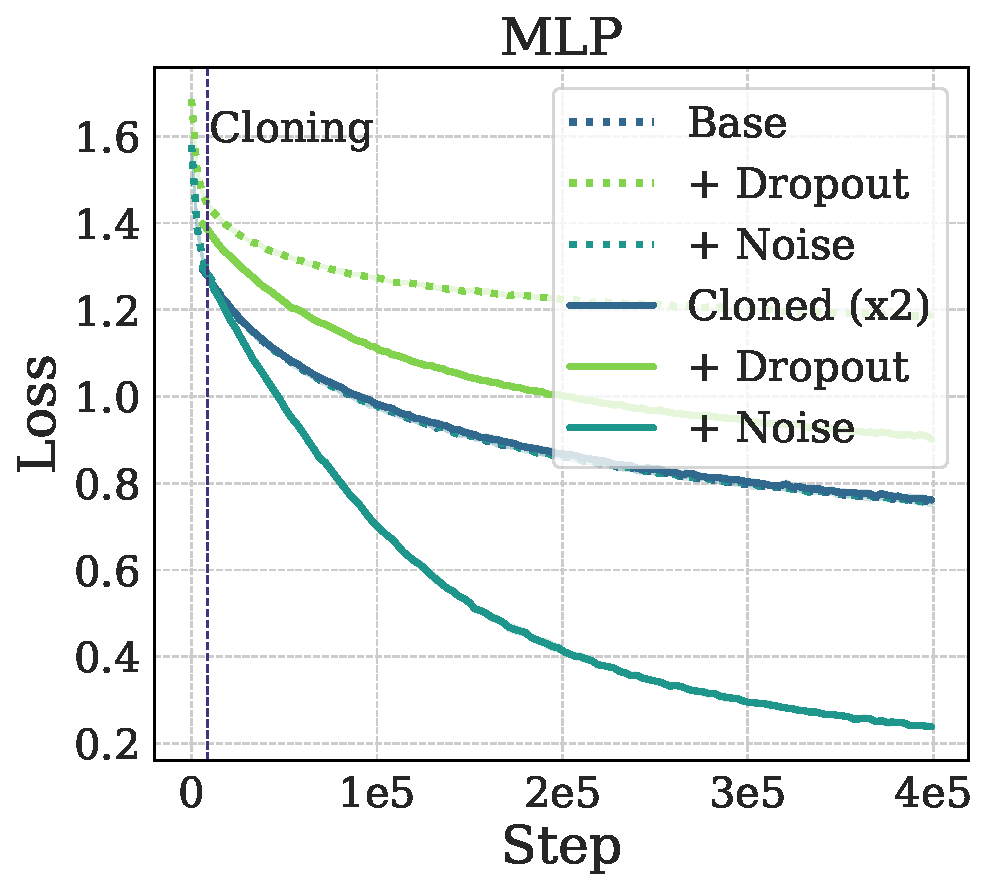
\includegraphics[height=12cm]{images/mlp_cloning_losses_plot.pdf}
\end{minipage}\hfill
\begin{minipage}[c]{0.47\linewidth}\centering
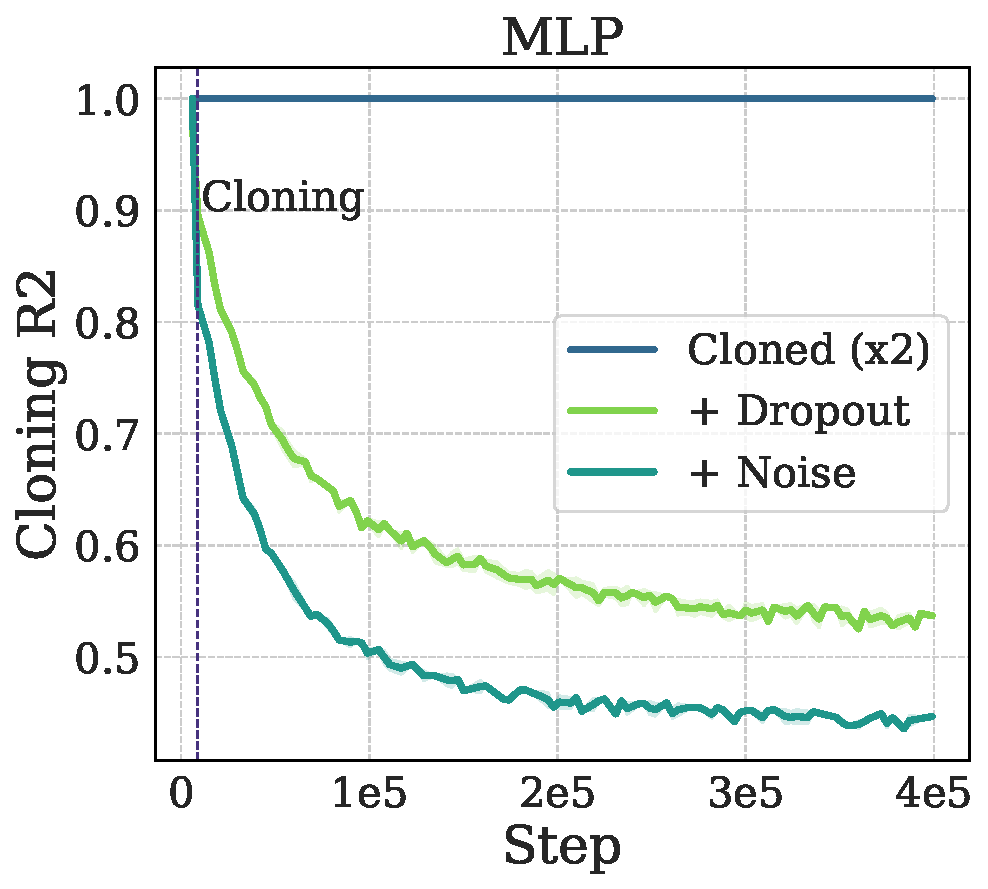
\includegraphics[height=12cm]{images/mlp_cloning_r2_plot.pdf}
\end{minipage}

\vspace{4mm}

% ROW 2: The Escape (Ablations)
\begin{minipage}[c]{0.47\linewidth}\centering
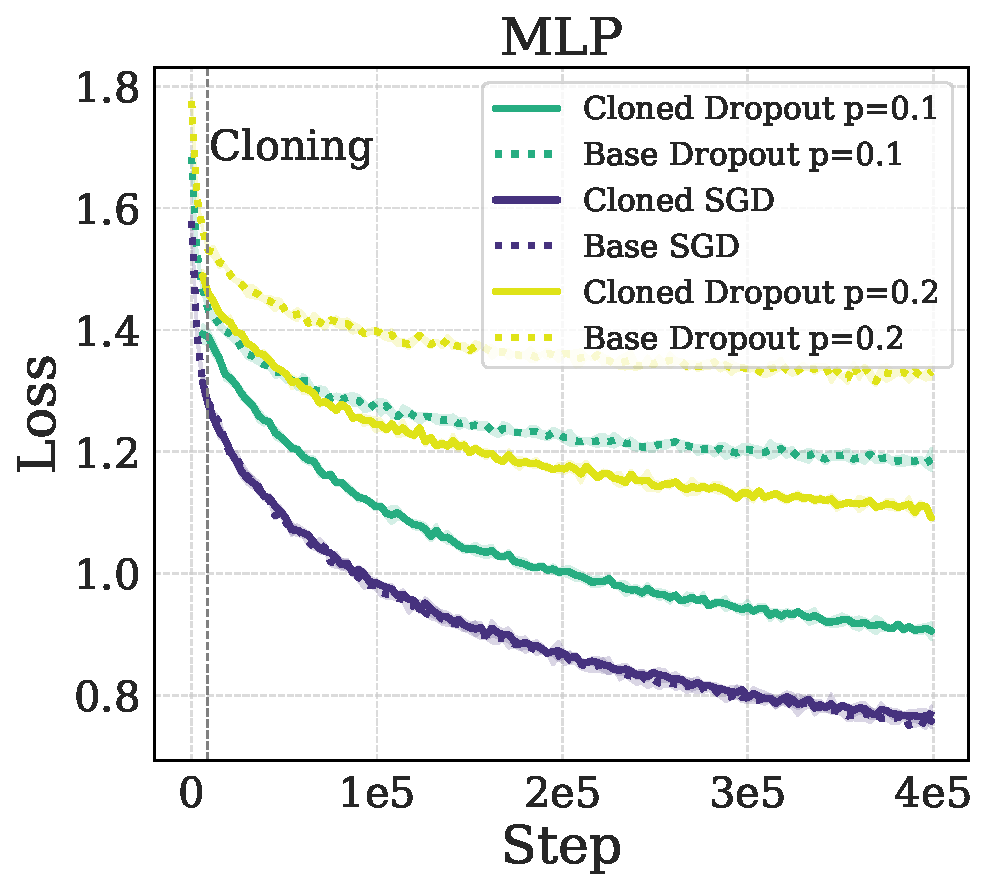
\includegraphics[height=12cm]{images/mlp_dropout_cloning_losses_plot.pdf}
\end{minipage}\hfill
\begin{minipage}[c]{0.47\linewidth}\centering
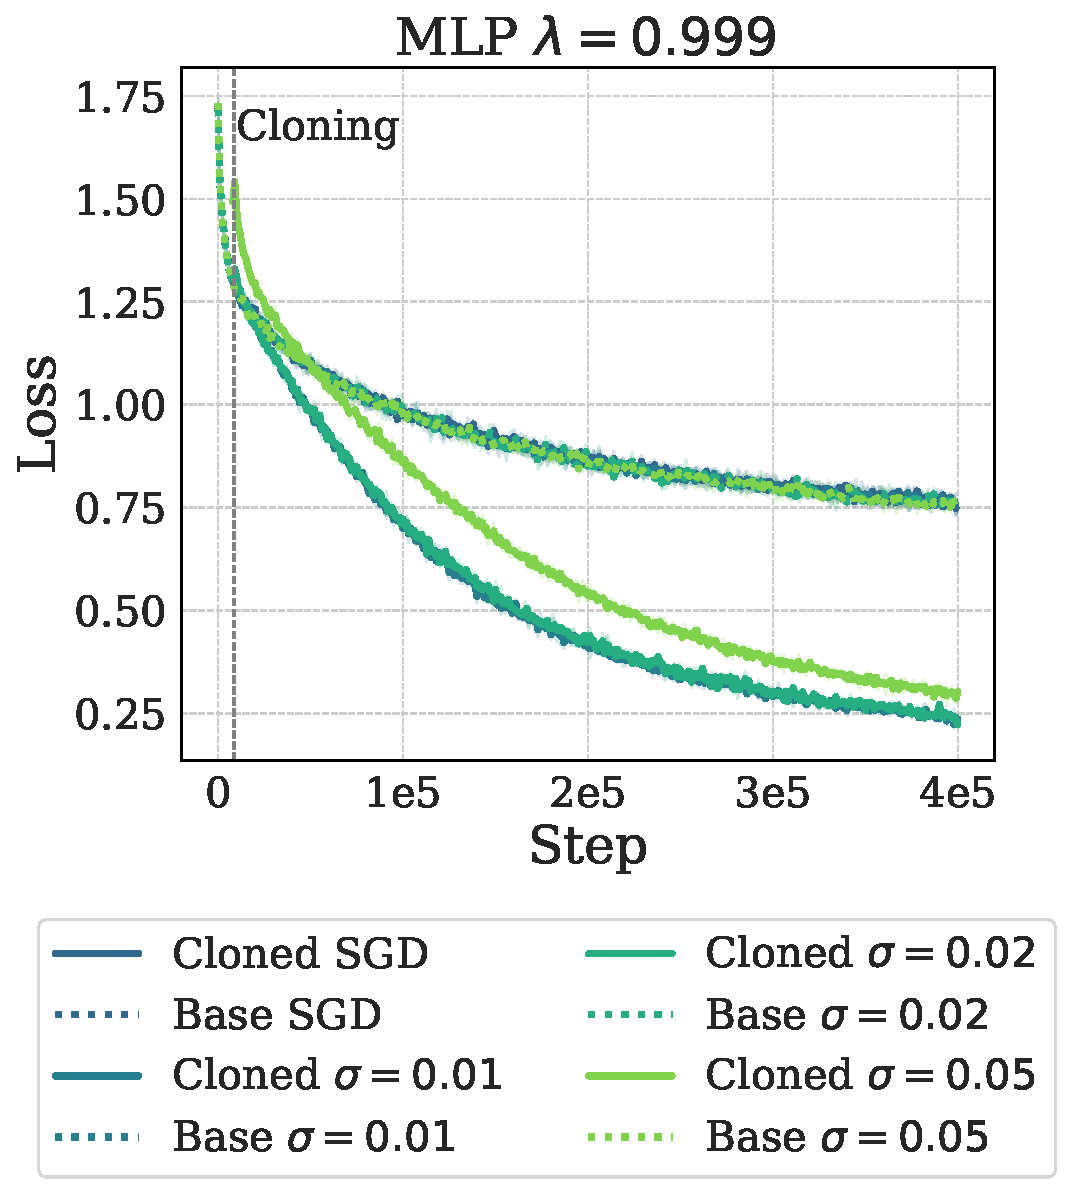
\includegraphics[height=12cm]{images/mlp_noises_cloning_losses_plot_sigma_lambda_0.999.png}
\end{minipage}
\end{center}

\vspace{2mm}
{\normalsize\color{tertiary} \textbf{Top Row (The Trap):} Without interventions, SGD and Adam are permanently trapped in the subspace ($R^2=1.0$). \textbf{Bottom Row (Ablations):} Breaking the geometric symmetry requires targeted perturbations. Increasing Dropout probability (left) or injected Noise scale (right) directly dictates the rate of escape.}
}

% \block{\textbf{2. The Mechanics: Exact Traps (Thm 1)}}{
% \large

% For a LoP manifold $\mathcal{M}\subseteq \Theta$, is \textbf{distribution-independent}, in the sense that for virtually all feasible inputs, regardless of their semantics, the gradient is tangent to the manifold.

% \thinrule

% \seclabel{Frozen-unit manifold \;$\mathcal{M}_F$}
% If units $F\subset V$ are persistently saturated ($f'(z_v(x;\theta))=0$), their incoming gradients vanish for every sample. $\mathcal{M}_F=\bigl\{\theta:\theta_{\mathrm{in}}(v)=\mathrm{const},\ \forall v\in F\bigr\}$.

% \vspace{2mm}
% {\color{frozen}\rule{14pt}{1.8pt}}\;\; \emph{A frozen unit is permanently silent to backprop.}

% \thinrule

% \seclabel{Cloning manifold \;$\mathcal{M}_C$}
% If block pairs satisfy equal row and column sums:
% \[
% \textstyle\sum_{v\in S_j}\theta_{uv}=\sum_{v\in S_j}\theta_{u'v},
% \quad
% \sum_{u\in S_i}\theta_{uv}=\sum_{u\in S_i}\theta_{uv'},
% \]
% then forward values $h_u(x)=h_{u'}(x)$ and backward errors $\delta_v(x,y)=\delta_{v'}(x,y)$ are strictly identical.

% \vspace{2mm}
% {\color{cloned}\rule{14pt}{1.8pt}}\;\; \emph{Cloned directions are indistinguishable to both passes.}

% \thinrule

% \resultbox{%
% \textbf{Degeneracy in computation induces degeneracy in the update:}
% $(h,\delta) \text{ degenerate} \Rightarrow \text{gradient degenerate} \Rightarrow \nabla_\theta \ell \in \T\mathcal{M}$
% }

% \thinrule

% \seclabel{Empirical Proof: Traps Confine SGD \& Adam}
% Do these theoretical locks hold? Yes. If initialized exactly on the cloning manifold, \textbf{counter-intuitively, even Adam is perfectly confined} despite parameter-wise gradient history. 

% \vspace{3mm}
% \begin{center}
% \begin{minipage}[c]{0.40\linewidth}\centering
% 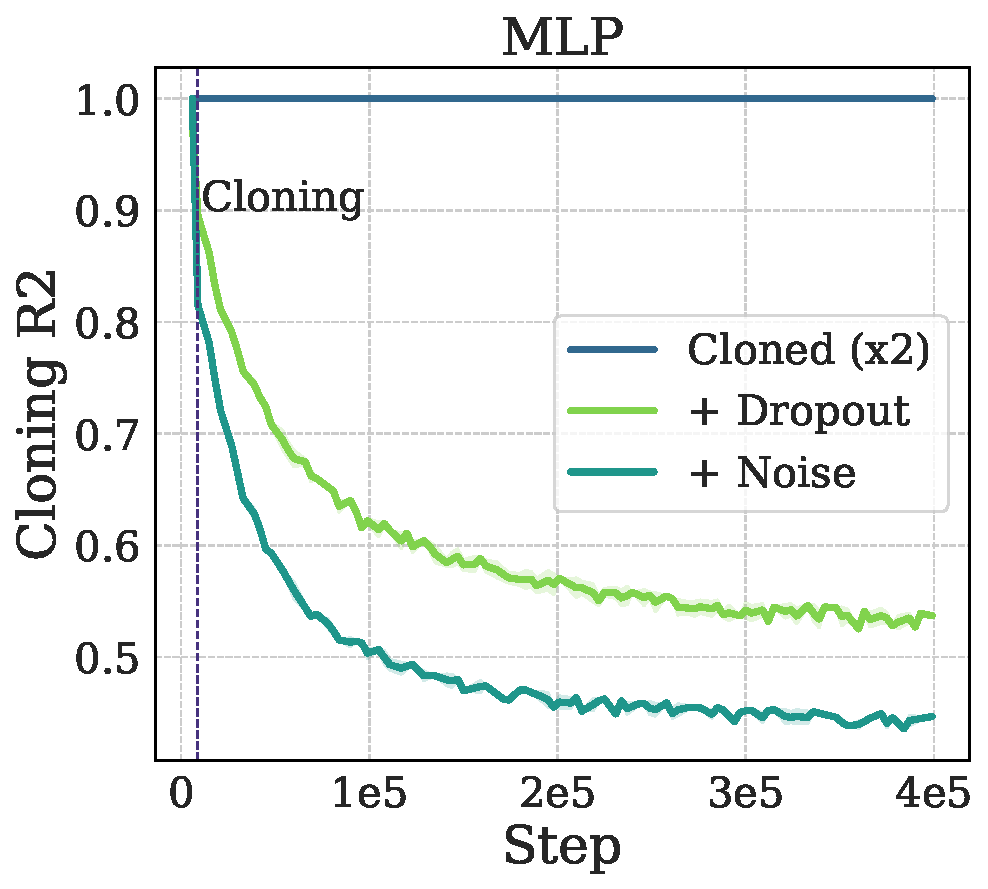
\includegraphics[width=\linewidth]{images/mlp_cloning_r2_plot.pdf}
% \end{minipage}\hspace{4mm}
% \begin{minipage}[c]{0.40\linewidth}\centering
% 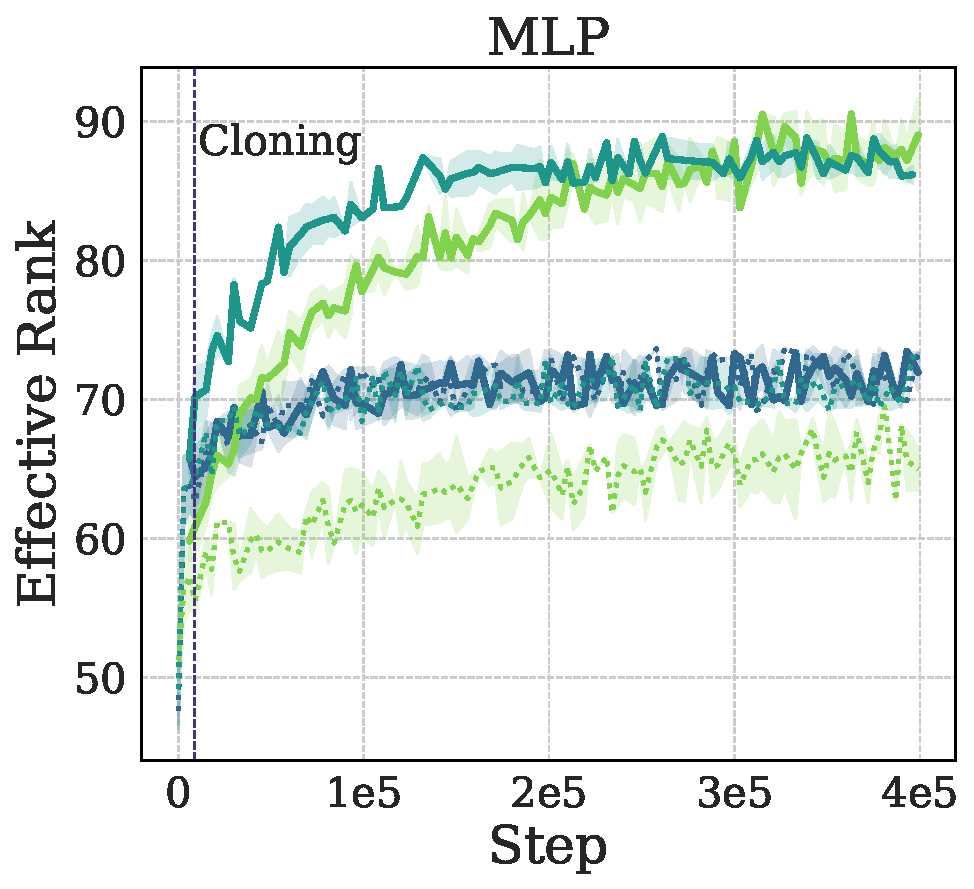
\includegraphics[width=\linewidth]{images/mlp_cloning_rank_plot.pdf}
% \end{minipage}
% \end{center}
% \vspace{1mm}
% {\normalsize\color{tertiary} Left: $R^2=1.0$ indicates perfect cloning (zero escape) for SGD and Adam. Right: Rank collapses. Escape requires explicit symmetry breaking (Dropout, Noise).}
% }

% ──────────────────────────────────────────────────────────────────
% COLUMN 3 — The Cause (Theorem 2) & The Cure
% ──────────────────────────────────────────────────────────────────
\column{0.34}

\block{\textbf{3. The Cause: Rank-Plasticity Tension}}{
\large
Training balances \textbf{compression} for generalization and \textbf{nonlinear feature creation}. \emph{The very mechanisms that help a model generalize on a static task actively drive it into LoP manifolds.}

% \thinrule

\seclabel{Rank-gain theorem (Theorem 2)}
Let $C$ be the \textbf{pre-activation} correlation matrix, and $K_{\mu,\sigma}(C)$ the \textbf{post-activation} correlation, modulated by pre-activation mean $\mu$ and std $\sigma$.

\vspace{2mm}
\[
\frac{\er\!\bigl(K_{\mu,\sigma}(C)\bigr)}{\er(C)} \;\ge\; 1 + \textcolor{frozen}{\underbrace{\gamma(\mu,\sigma)}_{\text{Strength}}} \cdot \textcolor{cloned}{\underbrace{\frac{\Psi(C)}{\|C\|_F^2}}_{\text{Potential}}}
\]
\vspace{2mm}

\resultbox{
\begin{center}
\textbf{\textcolor{frozen}{Activation Strength:}}\; $\bm{\gamma(\mu,\sigma) = \frac{1-K_{\mu,\sigma}'(0)}{1+K_{\mu,\sigma}'(0)}}$ \\[3mm]
\textbf{\textcolor{cloned}{Decorrelation Potential:}}\; $\bm{\Psi(C) = \sum_{i \ne j} C_{ij}^2(1-C_{ij}^2)}$
\end{center}
}

% \vspace{3mm}
% \seclabel{Two routes to LoP}
\begin{itemize}[leftmargin=1.4em, itemsep=2mm, topsep=1mm]
\item \textbf{\textcolor{frozen}{Frozen Trap ($\mathcal{M}_F$):}} Maximizing $\gamma(\mu,\sigma) \to 1$ requires saturation 
%(e.g., large negative bias). This drives units into regimes where gradients vanish ($f' \approx 0$).
\item \textbf{\textcolor{cloned}{Cloned Trap ($\mathcal{M}_C$):}} TO compress rank, correlations are forced to $C_{ij} \in \{0,\pm 1\}$ .
\end{itemize}

\vspace{2mm}
\begin{center}
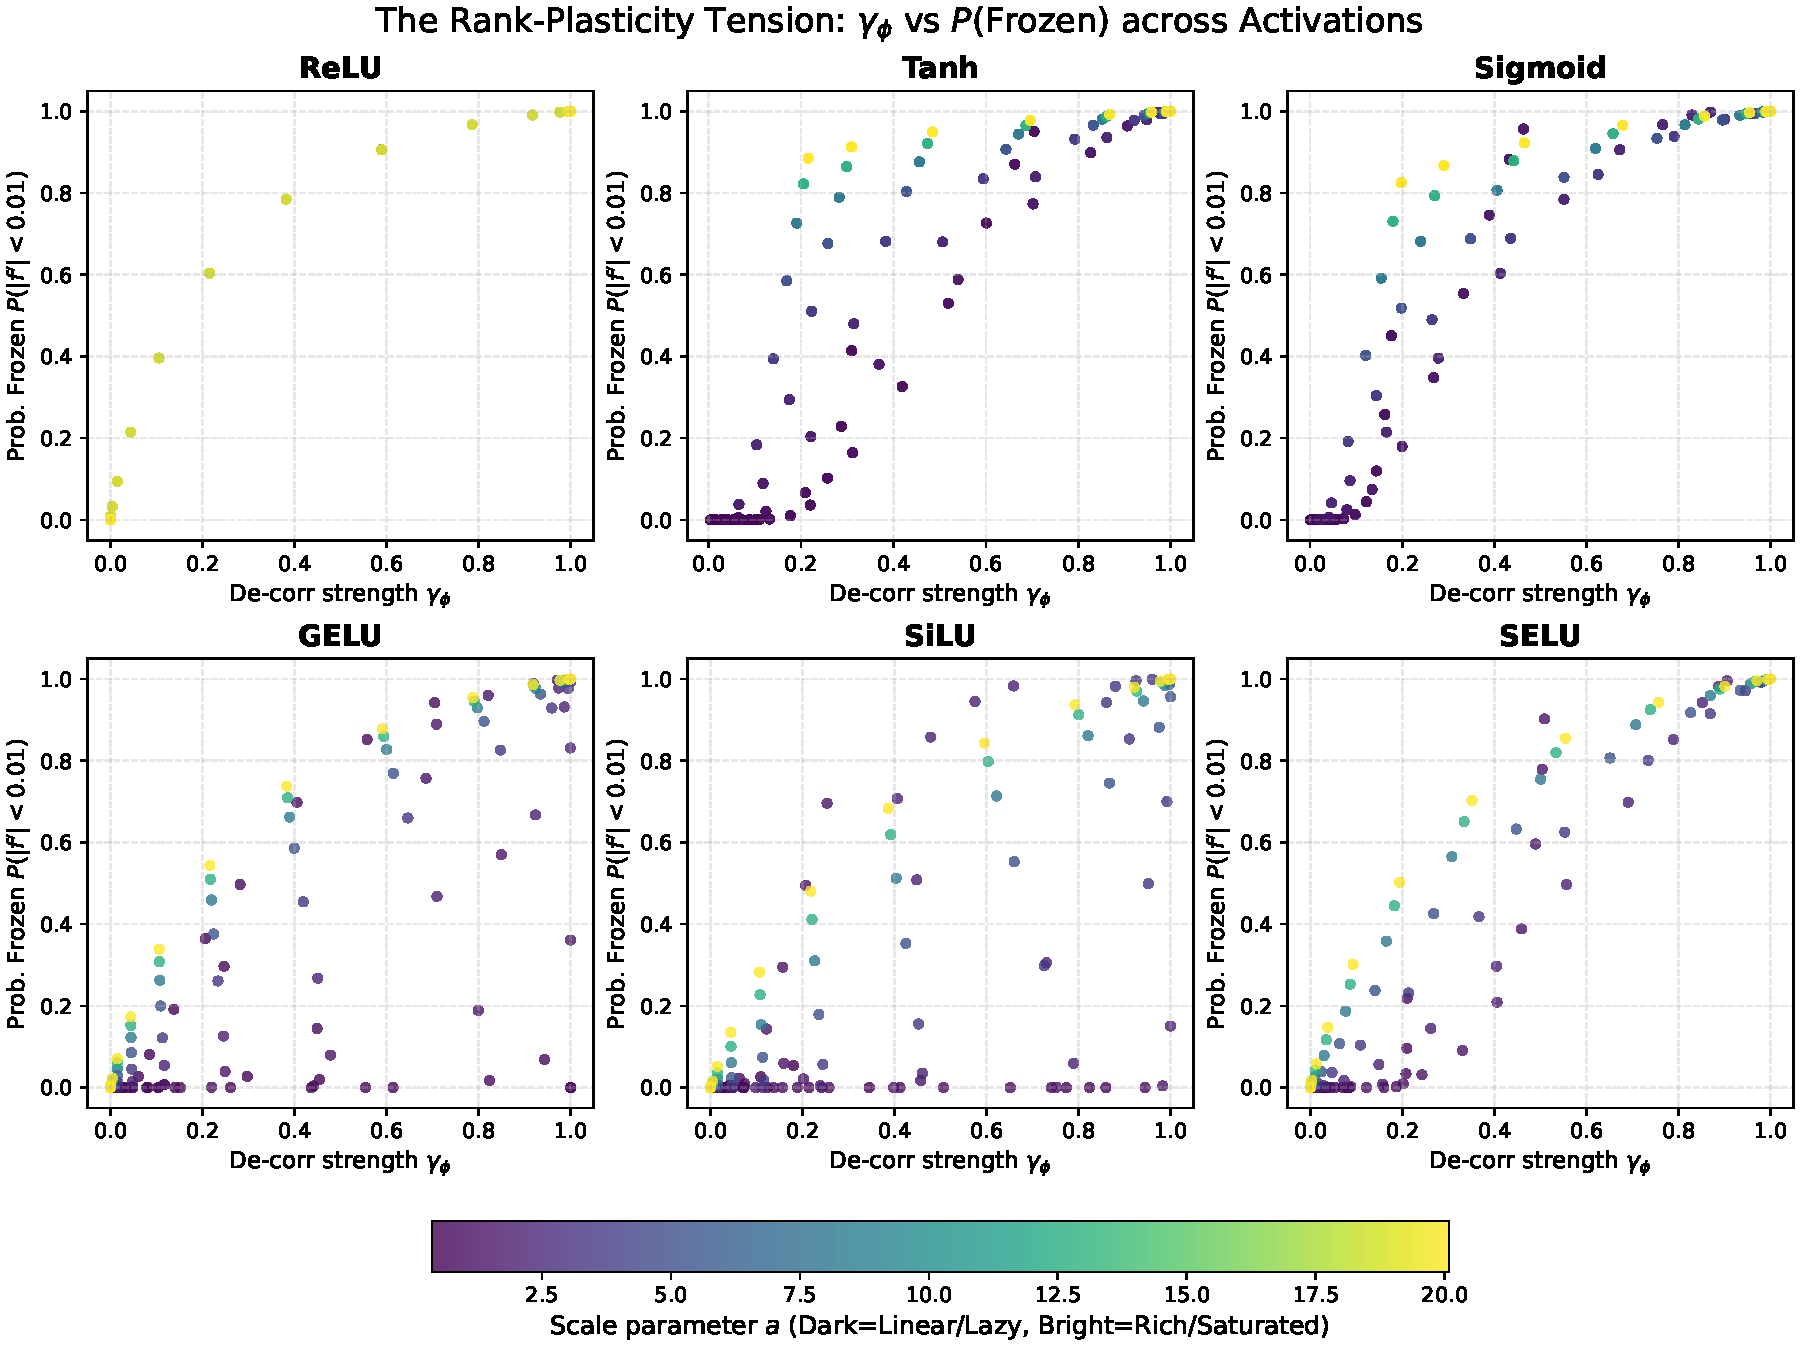
\includegraphics[width=0.35\linewidth, trim=290 350 290 20, clip]{images/universal_lop_plot.pdf}
\end{center}
\vspace{-1mm}
{\color{tertiary} Sweeping pre-activation $\mu, \sigma$ shows that maximizing $\gamma(\mu,\sigma)$ pushes activations towards freezing.}
}

% \block{\textbf{3. The Cause: Rank-Plasticity Tension}}{
% \large
% Training balances \textbf{compression} (for generalization) and \textbf{nonlinear creation} (for feature diversity). \emph{The very mechanisms that help a model generalize on a static task actively drive it into LoP manifolds.}

% \thinrule

% \seclabel{Rank-gain theorem (Theorem 2)}
% Study one linear--nonlinear stage. Let $\er(M)=\frac{(\mathrm{tr}\,M)^2}{\|M\|_F^2}$. Let $\gamma$ be decorrelation strength, and $\Psi$ be decorrelation potential. 

% \[
% \frac{\er\!\bigl(K_{\mu,\sigma}(C)\bigr)}{\er(C)} \;\ge\; 1+{\color{frozen}\gamma(\mu,\sigma)}\frac{{\color{cloned}\Psi(C)}}{\|C\|_F^2}
% \]

% \vspace{2mm}

% \resultbox{
% \begin{center}\textbf{Feature creation\; =\; {\color{frozen}strength}\; $\bm{\times}$\; {\color{cloned}remaining opportunity}}\end{center}
% }

% \vspace{3mm}
% \seclabel{Two routes to LoP}
% \begin{itemize}[leftmargin=1.4em, itemsep=1mm, topsep=1mm]
% \item \textbf{\textcolor{frozen}{Frozen Trap:}} ${\color{frozen}\gamma(\mu,\sigma)}\uparrow \;\Rightarrow\; \psi'_{\mu,\sigma}\approx 0 \;\Rightarrow\; \textcolor{frozen}{\mathcal{M}_F}$
% \item \textbf{\textcolor{cloned}{Cloned Trap:}} ${\color{cloned}\Psi(C)}\downarrow 0 \;\Rightarrow\; C_{ij}\in\{0,\pm1\} \;\Rightarrow\; \textcolor{cloned}{\mathcal{M}_C}$
% \end{itemize}

% \vspace{2mm}
% \begin{center}
% 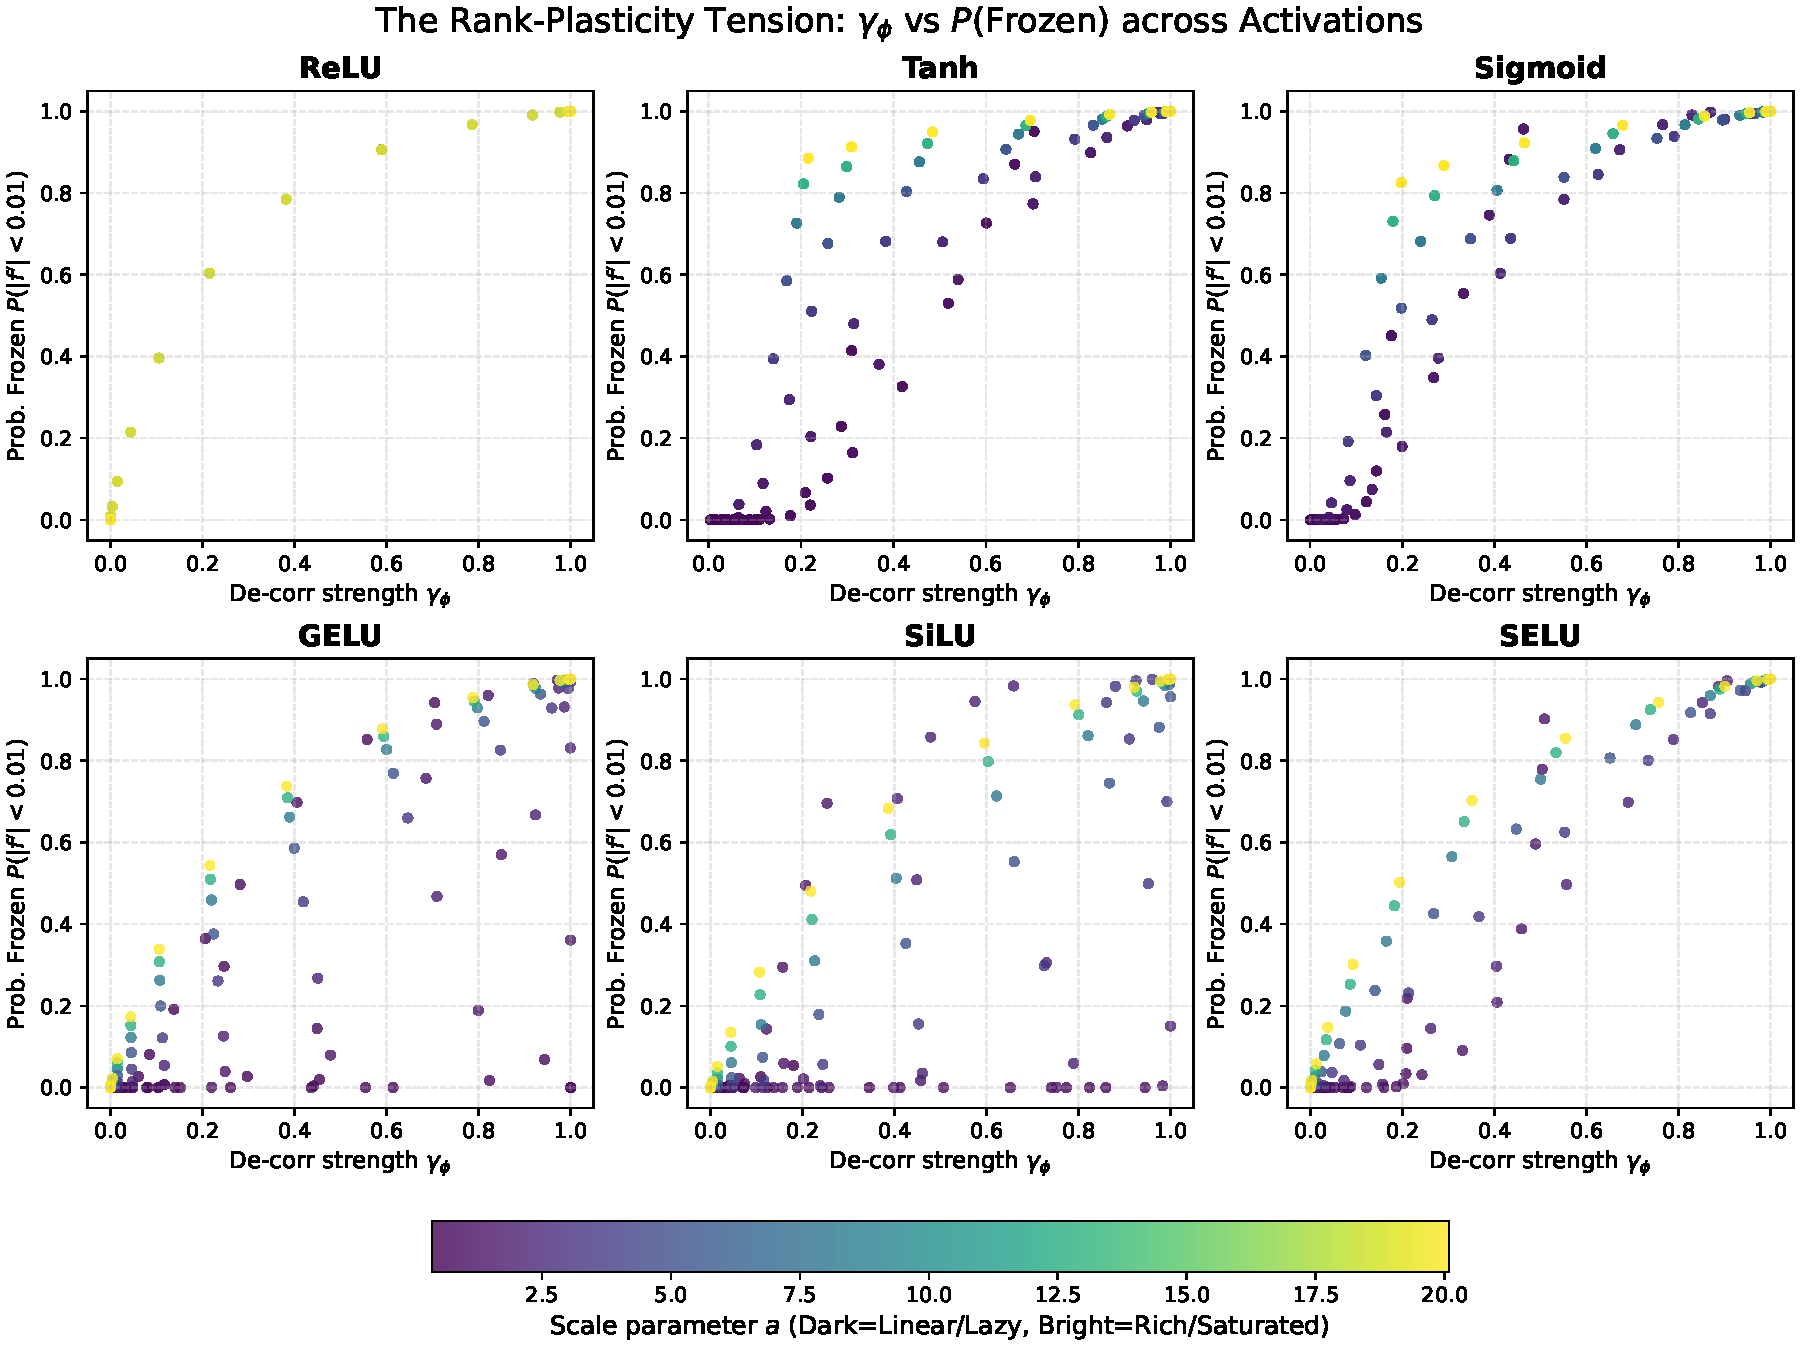
\includegraphics[width=0.85\linewidth, trim=0 380bp 0 30bp, clip]{images/universal_lop_plot.pdf}
% \end{center}
% \vspace{-1mm}
% {\small\color{tertiary} Regimes maximizing $\gamma_\phi$ simultaneously drive units toward freezing (across 6 activations).}
% }

\block{\textbf{4. Mitigation, Recovery \& Takeaway}}{
\large
\textbf{Continual BackProp} (CBP) escapes the \textcolor{cloned}{$\mathcal{M}_C$} cloned trap via targeted noise. \textbf{Normalization layers} bound pre-activation drift, preventing the \textcolor{frozen}{$\mathcal{M}_F$} frozen trap.

% \vspace{2mm}
\begin{center}
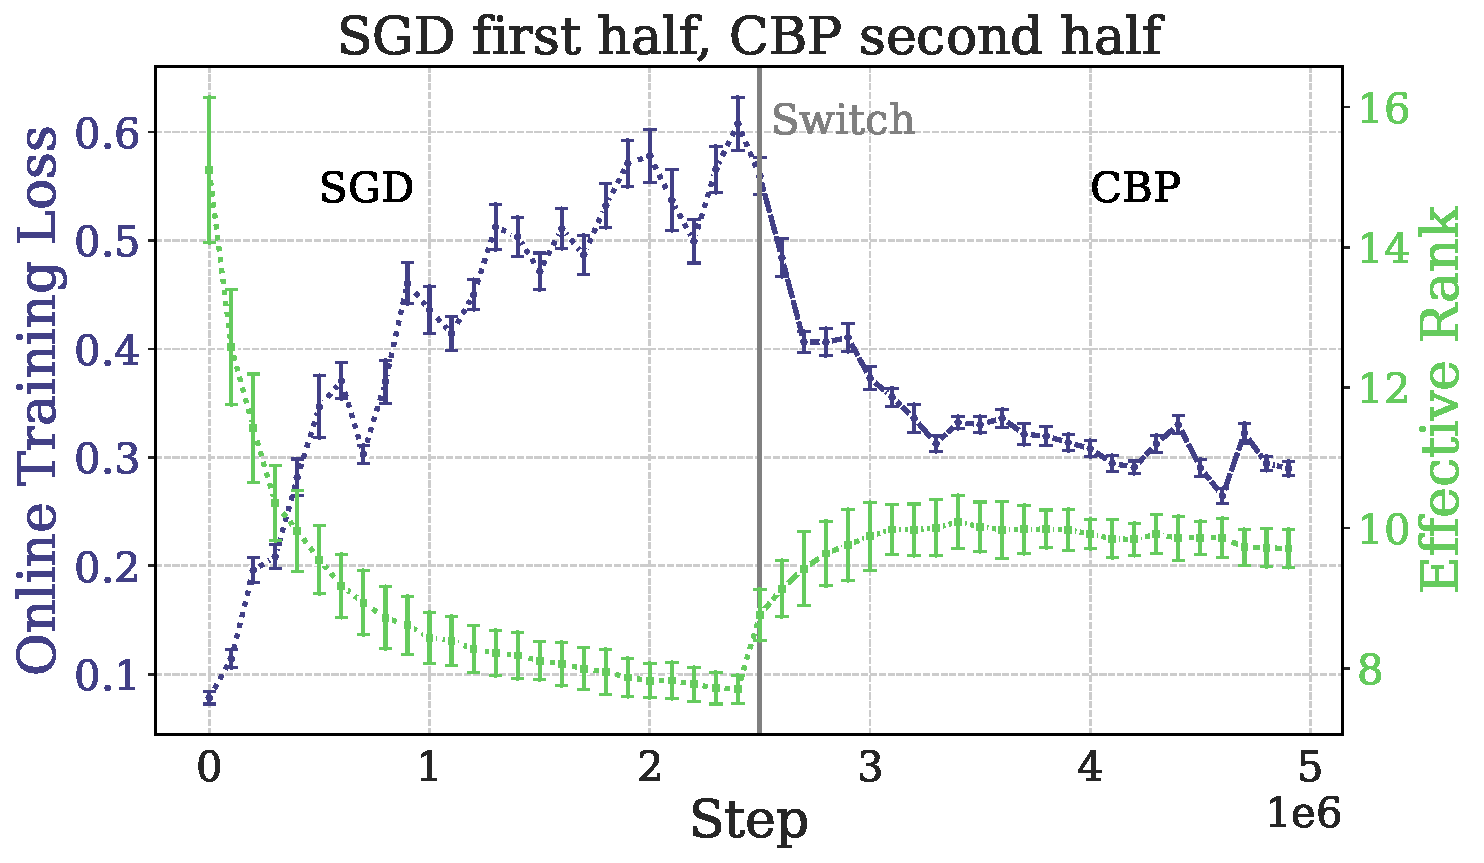
\includegraphics[height=11cm]{images/bf_switching_rankloss_plot.pdf}%
\hspace{3mm}%
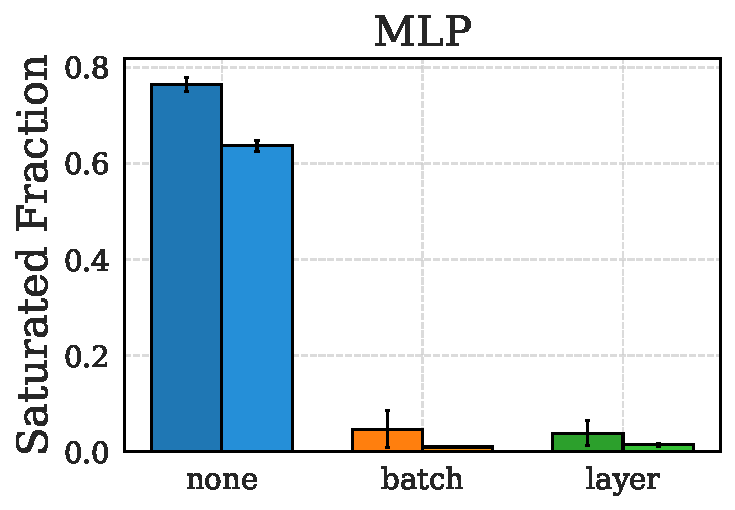
\includegraphics[height=11cm]{images/mlp_act__saturated_frac_normalizations_barplot.pdf}
\end{center}

% \vspace{2mm}
\takeawaybox{%
\textbf{Overall picture.\;}
\emph{Feature dynamics}
$\Rightarrow$
\emph{frozen/cloned structures}
$\Rightarrow$
\emph{LoP manifolds}
$\Rightarrow$
\textbf{Loss of plasticity.}
\textcolor{escape!80!black}{\textbf{Escape requires symmetry breaking (CBP, Dropout) or Normalization.}}
}

\vspace{3mm}
\begin{center}
\begin{tabular}{c@{\hspace{8mm}}c}
\qrcode[height=3.2cm]{https://github.com/ajoudaki/loss-of-plasticity} &
\qrcode[height=3.2cm]{https://openreview.net/forum?id=g6kof5fSba} \\[2mm]
{\normalsize\color{tertiary}\textbf{Code}} &
{\normalsize\color{tertiary}\textbf{Paper}}
\end{tabular}
\hspace{30mm}
\raisebox{1mm}{
\includegraphics[height=15mm]{elements/eth_logo_kurz_pos}}
\hspace{20mm}%
\raisebox{1mm}{\fontsize{55}{55}\selectfont\faApple}%
\end{center}

\vspace{2mm}
{\color{separator}\hrule height 0.4pt}
\vspace{2mm}
{\scriptsize\color{tertiary}
{[1]} Abraham \& Robins, \emph{Neurocomp.}, 2005.\quad
{[2]} Chaudhry et al., \emph{ECCV}, 2018.\quad
{[3]} Dohare et al., \emph{Nature}, 2024.\quad
{[4]} Lyle et al., \emph{ICML}, 2023.\quad
{[5]} Sokar et al., \emph{NeurIPS}, 2023.\quad
{[6]} Nikishin et al., \emph{NeurIPS}, 2022.%
}
}

\end{columns}

\end{document}